\section{Interpolation with Shifted Symmetric Functions}\label{sec:p5}

\begin{enumerate}[(a)]
\item We are given the coefficients $\{c[k]\}$, so
\begin{align*}
	s(t) &= \sum_{k \in \mathbb{Z}} c[k] \phi (t-kT)\\
	\Rightarrow s(nT) &= x[n] = \sum_{k \in \mathbb{Z}}c[k] \phi(nT-kT) \\
	&= \sum_{k \in \mathbb{Z}} c[k] \phi((n-k)T) \\
	&= \sum_{k \in \mathbb{Z}} c[k] b[n-k]
\end{align*}
where $b[m] = \phi(mT)$. So
\[x = c * b \Rightarrow X(z) = C(z)B(z) \Rightarrow C(z) = \frac{1}{B(z)}X(z) = H(z)X(z)\]
where $H(z) = \frac{1}{B(z)}$.

%To enable this, we require $B(z) \neq 0 \Leftrightarrow \phi(jT) \neq 0, \forall j$.
To enable this, we need $\phi(nT)$ to be band limited in the range of $[\frac{-\pi}{T}, \frac{\pi}{T}]$ to avoid aliasing.

\item If $\phi(t) = \phi(-t)$, then
\begin{align*}
	\phi(jT) &= \phi(-jT) \\
	\Leftrightarrow b[j] &= b[-j]
\end{align*}
If $\lambda$ is a pole/root of $H(z)$ then $B(\lambda) = 0$. We have
\begin{align*}
	B(z^{-1})
	&= \sum_{n=-N}^{N} b[n] z^n \\
	&= \sum_{n=-N}^{N} b[-n] z^n \\
	&= \sum_{m=-N}^{N} b[m] z^{-m} \qquad \because m = -n \\
	&= B(z)
\end{align*}
Therefore $\lambda^{-1}$ is also a root of $H(z)$.

\item Assume that $\lambda_j$ is a pole of $H(z)$, then $z = \lambda_j \Rightarrow 1-\lambda_j z^{-1} = 0$. Since $\lambda_j^{-1}$ is also a pole, $z = \lambda_j^{-1} \Rightarrow 1 - \lambda_j z = 0$. Therefore, we can write $H(z)$ as

\[H(z)= \frac{1}{\prod_j (1-\lambda_j z^{-1})} \cdot \frac{1}{\prod_j (1-\lambda_jz)}\]
Let $G(z) = \frac{1}{\prod_j (1-\lambda_j z^{-1})}$ (causal), then $G(z^{-1}) = \frac{1}{\prod_j (1-\lambda_j z)}$. Hence, \[H(z) = G(z)G(z^{-1}), \qquad \text{with } G(z) = \frac{1}{\prod_j (1-\lambda_j z^{-1})}\]

\item We can see that
\begin{align*}
(1 - \lambda_1 z^{-1}) &= 1 - \lambda_1 z^{-1} \\
(1 - \lambda_1 z^{-1})&(1 - \lambda_2z^{-1}) \\ &= 1 - (\lambda_1 + \lambda_2)z^{-1} + \lambda_1 \lambda_2 z^{-2} \\
(1 - \lambda_1 z^{-1})&(1 - \lambda_2 z^{-1})(1 - \lambda_3 z^{-1}) \\ &= (1 - (\lambda_1 + \lambda_2)z^{-1} + \lambda_1 \lambda_2 z^{-2})(1 - \lambda_3 z^{-1}) \\
&= 1 - (\lambda_1 + \lambda_2 + \lambda_3)z^{-1} + (\lambda_1\lambda_2 + \lambda_1\lambda_3 + \lambda_2\lambda_3)z^{-2} - \lambda_1\lambda_2\lambda_3 z^{-3} \\
\cdots
\end{align*}
Therefore, in general
\[\prod_{j=1}^{M} (1-\lambda_j z^{-1}) = \sum_{j=0}^M \xi_j z^{-j}\]
where $\xi_j = (-1)^j \zeta_j$ and $\zeta_j$ is the sum of products of $j$ elements from the set $\{\lambda_1, \cdots, \lambda_M\}$ (Vieta's formula), i.e.
\[\begin{cases}
\zeta_1 = \lambda_1 + \lambda_2 + ... \lambda_M \\
\zeta_2 = (\lambda_1\lambda_2 + \lambda_1\lambda_3 + ... + \lambda_1\lambda_M) + (\lambda_2\lambda_3 + \lambda_2\lambda_4 + ... + \lambda_2\lambda_M) + ... + \lambda_{M-1}\lambda_M \\
\vdots \\
\zeta_M = \lambda_1 \lambda_2 ... \lambda_M 
\end{cases}\]

Since $H(z) = G(z)G(z^{-1})$
\begin{align*}
Y(z) 
&= X(z)H(z) \\
&= X(z)G(z)G(z^{-1})
\end{align*}
Let $V(z) = X(z)G(z)$, we can sketch a diagram of the system as in Figure \ref{fig:p5d}

%We notice that $G(z)$ is an IIR filter, so we can use direct form I to sketch $G(z)$ and $G(z^{-1})$ is sketched by replacing $z{-1}$ blocks in $G(z)$ by $z$ blocks (Figure \ref{fig:p5d}).

\begin{figure}[htbp]
	\centering
	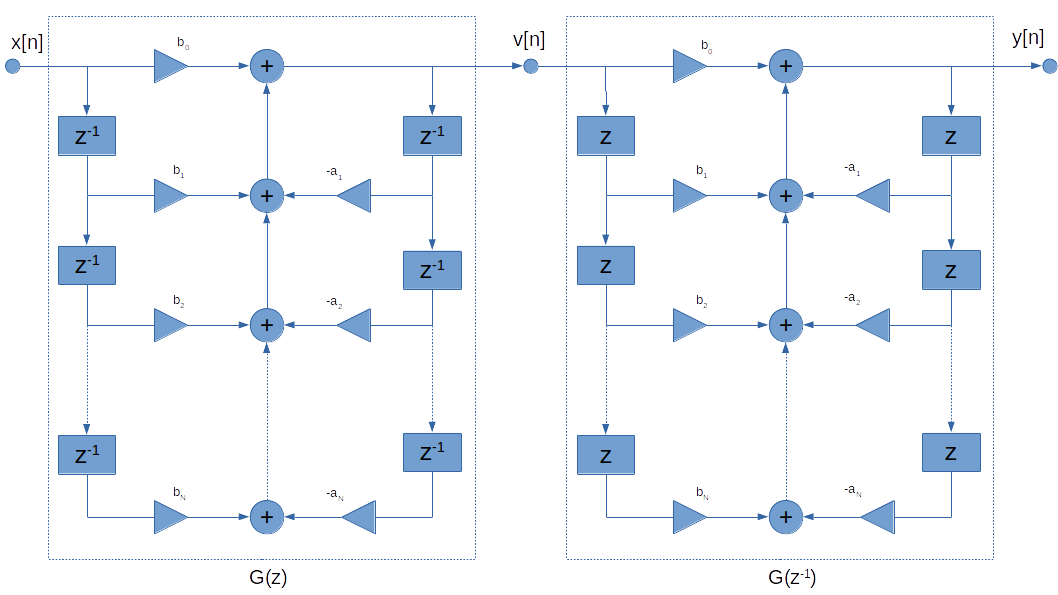
\includegraphics[width=\linewidth]{images/p5d}
	\caption{$H(z)$ as a cascade of causal $G(z)$ and anti-causal $G(z^{-1})$}
	\label{fig:p5d}
\end{figure}
\end{enumerate}